% MSRI - SGS Sparsity week 1, Wednesday, 1 lecture, 60 minutes

\documentclass{beamer}

\usepackage{amsmath,amssymb,amsthm,mathrsfs,amscd,mathtools}
\usepackage{datetime}
\usepackage{csquotes}
\usepackage{hyperref}
\usepackage{graphicx}
\usepackage{tikz,tikz-cd}
\usetikzlibrary{arrows,shapes}

\usetheme{Metropolis}
\metroset{block=fill}




\newcounter{maincounter}
\newcounter{excounter}

\newtheorem{conjecture}{Conjecture}
% \setbeamercolor{block body}{bg=mDarkTeal!15}
% \setbeamercolor{block title}{bg=mDarkTeal,fg=black!2}


\newcounter{maincounter}
\newcounter{excounter}
\numberwithin{maincounter}{chapter}
\numberwithin{equation}{chapter}
\numberwithin{excounter}{chapter}
\renewcommand{\theexcounter}{\thechapter.\Alph{excounter}}
\newtheorem{lemma}[maincounter]{Lemma}
\newtheorem{proposition}[maincounter]{Proposition}
\newtheorem{corollary}[maincounter]{Corollary}
\newtheorem{remark}[maincounter]{Remark}
\newtheorem{theorem}[maincounter]{Theorem}
\newtheorem{exercise}[excounter]{Exercise}
\newtheorem{example}[maincounter]{Example}

\newtheorem*{crucial}{Crucial Observation}

\newtheorem{conjecture}[maincounter]{Conjecture}
\newtheorem{definition}[maincounter]{Definition}

\def\AA{\mathbb{A}}
\def\BB{\mathbb{B}}
\def\EE{\mathbb{E}}
\def\HH{\mathbb{H}}
\def\DD{\mathbb{D}}
\def\NN{\mathbb{N}}
\def\RR{\mathbb{R}}
\def\TT{\mathbb{T}}
\def\CC{\mathbb{C}}
\def\ZZ{\mathbb{Z}}
\def\PP{\mathbb{P}}
\def\QQ{\mathbb{Q}}
\def\FF{\mathbb{F}}
\def\GG{\mathbb{G}}
\def\LL{\mathbb{L}}
\def\MM{\mathbb{M}}
\def\SS{\mathbb{S}}
\def\UU{\mathbb{U}}
\def\XX{\mathbb{X}}


%%% Philipp's macros

\newcommand{\dom}[1]{{\mathrm {dom}}({#1})}
\newcommand{\sman}[1]{{#1}^{\mathrm{sm,an}}}
\newcommand{\ansm}[1]{{#1}^{\mathrm{an,sm}}}
\newcommand{\sm}[1]{{#1}^{\mathrm{sm}}}
\newcommand{\anE}{\mathrm{an}}
\newcommand{\an}[1]{{#1}^{\anE}}
\newcommand{\stab}[1]{{\mathrm{Stab}(#1)}}


\newcommand{\hgtexp}{S}

\newcommand{\rank}{{\rm rank}\,}
\newcommand{\Hpoly}[2]{{H^{}_{#1}({#2})}}
\newcommand{\poly}[2]{{#1^{}({#2})}}
\newcommand{\polyt}[2]{{#1^{\sim}({#2})}}
\newcommand{\polytiso}[2]{{#1^{\sim,{\rm iso}}({#2})}}
%\renewcommand{\graph}[1]{\Gamma({#1})}
\newcommand{\atopx}[2]{{\genfrac{}{}{0pt}{}{#1}{#2}}}
\newcommand{\IP}{{\PP}}
\newcommand{\IG}{{\GG}}
\newcommand{\IH}{{\HH}}
\newcommand{\IC}{{\CC}}
\newcommand{\IR}{{\RR}}
\newcommand{\IT}{{\TT}}
\newcommand{\IRan}{{{\RR}_{\rm an}}}
\newcommand{\IRanexp}{{{\RR}_{\rm an,exp}}}
\newcommand{\RRan}{{\IRan}}
\newcommand{\RRanexp}{{\IRanexp}}
\newcommand{\IRalg}{{\RR}_{\rm alg}}
\newcommand{\IQbar}{{\overline{\QQ}}}
\newcommand{\Kbar}{{\overline{K}}}
\newcommand{\IZ}{{\ZZ}}
\newcommand{\IN}{{\NN}}
\newcommand{\IA}{{\AA}}
\newcommand{\IQ}{{\QQ}}
\newcommand{\IQpbar}{{\overline{\QQ}_p}}
\newcommand{\IQp}{{\QQ_p}}
\newcommand{\ts}[1]{{T}_0({#1})}

\newcommand{\cC}{{\mathcal C}}
\newcommand{\cE}{{\mathcal E}}
\newcommand{\cF}{{\mathcal F}}
\newcommand{\cK}{{\mathcal K}}
\newcommand{\cL}{{\mathcal L}}
\newcommand{\cM}{{\mathcal M}}
\newcommand{\cO}{{\mathcal O}}
\newcommand{\cV}{{\mathcal V}}
\newcommand{\cW}{{\mathcal W}}
\newcommand{\cX}{{\mathcal{X}}}
\newcommand{\cY}{{\mathcal Y}}
\newcommand{\cZ}{{\mathcal Z}}



\newcommand{\defZ}{Z}
\newcommand{\defF}{F}
\newcommand{\defW}{W}
\newcommand{\defC}{C}
\newcommand{\defE}{E}
%\newcommand{\deffam}{F}


\newcommand{\re}[1]{{\rm Re}({#1})}
\newcommand{\imS}{{\rm Im}}
\newcommand{\im}[1]{\imS({#1})}
\newcommand{\imageS}{{\rm im}}
\newcommand{\image}[1]{\imageS({#1})}
\newcommand{\volS}{{\rm vol}}
\newcommand{\vol}[1]{\volS({#1})}
\newcommand{\orth}[1]{{#1}^{\bot}}
\newcommand{\mat}[2]{{\rm Mat}_{#1}({#2})}
\newcommand{\ssm}{\setminus}
\newcommand{\ord}[1]{{\rm ord}({#1})}
\newcommand{\opt}[2]{{\rm Opt}_{#2}({#1})}
\newcommand{\Height}[1]{{H}({#1})}
\newcommand{\trdeg}{{\rm trdeg\,}} 
\newcommand{\geo}[1]{\langle {#1}\rangle_{{\rm geo}}}
\newcommand{\defect}{\delta}
\newcommand{\geodef}{{\delta_{\rm geo}}}
\newcommand{\en}[1]{{\rm End}({#1})}
\newcommand{\Hom}[1]{{\rm Hom}({#1})}
\newcommand{\hommaxR}[1]{\text{\rm Hom}({#1})^{*}_{\IR}}
\newcommand{\arith}{\rm arith}
\newcommand{\sgu}[2]{{#1}^{[{#2}]}}
\newcommand{\oa}[1]{{#1}^{\rm oa}}
\newcommand{\codim}{{\rm codim}}
\newcommand{\lgo}{LGO}
\newcommand{\zcl}[1]{{\rm Zcl}({#1})}


\newcommand{\trans}[1]{{#1}^{T}}

\newcommand{\red}[1]{\textcolor{red}{#1}}

\renewcommand{\subset}{\subseteq} %%% Some people think \subset
%%% excludes equality
\renewcommand{\supset}{\supseteq}

\newcommand{\gra}[1]{\mathrm{Gr}({#1})}


\newcommand{\gl}[2]{{\mathrm {GL}}_{#1}({#2})}
\renewcommand{\sp}[2]{{\mathrm {Sp}}_{#1}({#2})}
\newcommand{\autS}{{\mathrm {Aut}}}
\newcommand{\aut}[1]{\autS({#1})}

\newcommand{\spec}[1]{\mathrm{Spec}\,{#1}}

\newcommand{\tor}[1]{{#1}_{\mathrm{tor}}}
\newcommand{\gal}[1]{{\mathrm{Gal}}({#1})}


\newcommand{\zeroset}[1]{\mathscr{Z}({#1})}


\newcommand{\jac}{\mathrm{Jac}}

\newcommand{\bfzeta}{{\boldsymbol{\zeta}}}

\newcommand{\mattt}[4]
{\left(
  \begin{array}{cc}
    {#1} & {#2} \\ {#3} & {#4} 
  \end{array}
\right)}

\newcommand{\matto}[2]
{\left(
  \begin{array}{c}
    {#1} \\ {#2}
  \end{array}
\right)}

\newcommand{\matot}[2]
{\left(
  \begin{array}{cc}
    {#1} & {#2}
  \end{array}
\right)}


\title{MSRI Summer Graduate School \\ Sparsity of Algebraic Points \\
  Day 3: Pila--Wilkie Theorem and Transcendence}
\author{Philipp~Habegger \\ University of Basel \\ \texttt{philipp.habegger@unibas.ch}}
\date{Wednesday, June 9, 2021}

\begin{document}

\setlength{\abovecaptionskip}{0pt} 
\setlength{\belowcaptionskip}{0pt} 

\renewcommand{\figurename}{Fig.}


\begin{frame}
  \titlepage
\end{frame}
\section{Preview}
\begin{frame}
  Let $A$ be an abelian variety defined over $\IC$ of dimension $g$. 
  \begin{definition}
    A \alert{torsion coset} $\cK$ of $A$
    the translate of an
    abelian subvariety of $A$ by a torsion point. So
    $$ \cK = T+B $$
    with $B$ an abelian subvariety of $A$ and $T$ a point of finite order. 
  \end{definition}

  Recall $A(\IC) = \IC^g / \Omega$ and there is a $\IZ$-basis
  $(\omega_1,\ldots,\omega_{2g})$ of $\Omega$, here $\IC^{g} \cong
  \mathrm{T}_0(A)$. 

  The group of torsion points $A_{\mathrm{tors}}$ is the image
  of $\omega_1\IQ+\cdots+\omega_{2g}\IQ$  in $A(\IC)$.

  Set $\Omega_B = \mathrm{T}_0(B)\cap \Omega$, then $B(\IC) =
  \mathrm{T}_0(B) / \Omega_B$.

  The torsion points of $T+P$ are
  \alert{dense} in $T+B$ (with respect to the Zariski \alert{and}
  Archimedean topology).   
\end{frame}

\begin{frame}
  \begin{theorem}[Manin--Mumford Conjecture, Raynaud]
    Let $V\subset A$ be an irreducible closed subvariety. Then
    \begin{equation*}
      V\cap A_{\mathrm{tors}} \text{ is Zariski closed in $V$}
      \Longleftrightarrow \text{$V$ is a torsion coset.}
    \end{equation*}
  \end{theorem}

  Let $C/\IC$ be a smooth projective curve of genus $g\ge 1$. Its
  \alert{Jacobian}
  $$\mathrm{Jac}(C):=\mathrm{Pic}^0(C)\cong
  \mathrm{Div}_0(C)/\text{(lin. equiv.)}$$
  is an abelian variety.

  Let $P_0\in C(\IC)$ be any base point. Then
  \begin{equation*}
    P\mapsto ([P]-[P_0])/\text{(lin. eqiuv.)} 
  \end{equation*}
  induces a closed immersion
  \begin{equation*}
    C\rightarrow \mathrm{Jac}(C).
  \end{equation*}
\end{frame}  

\begin{frame}{The Original Question of Manin and Mumford}
  \begin{theorem}[Manin--Mumford Conjecture, Raynaud]
    Let $V\subset A$ be an irreducible closed subvariety. Then
    \begin{equation*}
      V\cap A_{\mathrm{tors}} \text{ is Zariski closed in $V$}
      \Longleftrightarrow \text{$V$ is a torsion coset.}
    \end{equation*}
  \end{theorem}
  Many different proofs, including one by Pila--Zannier
  that uses \alert{o-minimal geometry} and the
    \alert{Pila--Wilkie Theorem}.

  \begin{corollary}
    Suppose
    $C$ is immersed in its Jacobian $\mathrm{Jac}(C)$. If $C(\IC)\cap
    \mathrm{Jac}(C)_{\mathrm{tors}}$ is infinite, then $g=1$. 
  \end{corollary}
  \begin{proof}
    A $1$-dimension torsion coset in an abelian variety must be a
    smooth projective curve of genus $1$. 
  \end{proof}
  \vspace{-.25cm}
  
  Our goal: prove the theorem in an important case.
\end{frame}

\section{The Pila--Wilkie Theorem}

\begin{frame}{The Height Function}
  \begin{definition}
    \begin{enumerate}
    \item [(i)]
      Let $x\in \IQ$. There exist coprime integers $p,q$ with
      $q\ge 1$ and $x=p/q$. The \alert{height} of $x$ is $H(x)=\max\{|p|,q\}$.
    \item[(ii)] Let $(x_1,\ldots,x_m)\in\IQ^m$. There exist coprime integers
      $p_1,\ldots,p_m,q$ with $q\ge 1$ and $x_i = p_i/q$ for all $i\in
      \{1,\ldots,m\}$.
      The  \alert{height},
      of $(x_1,\ldots,x_m)$ is $H(x_1,\ldots,x_m)
      = \max_{1\le i\le m} \{|p_1|,\ldots,|p_m|,q\}$.
    \end{enumerate}
  \end{definition}

  \begin{example}
  \begin{enumerate}
  \item [(i)] $H(-1)=H(1)=H(0)=0$ and $H(2021/2023) = 2023$.
  \item[(ii)] 
    $H(x^d)=H(x)^d$ if $d\ge 1$ and $x\in \IQ^\times \Rightarrow H(x)=H(1/x)$ 

  \item[(iii)] $x,y\in\IQ\Rightarrow H(xy)\le H(x)H(y)$ and $H(x+y)\le
    2H(x)H(y)$
  \item[(iv)] $H(1/2,1/3,1/5) = 30, H(8,4,2,1,1/2,1/4,1/8) = 64$
  \end{enumerate}  
  \end{example}
\end{frame}

\begin{frame}
  \begin{example}\label{ex:heightcount1}
    \begin{enumerate}
    \item [(i)] If $T\ge 1$, then the \alert{Northcott property} holds:  
      $$ \# \{ x\in \IQ^m : H(x)\le T\} <\infty.$$

    \item[(ii)]
      Set $N(T) = \#\{x\in\IQ : H(x)\le T\}$.
      If $T\ge 1$ is an integer, then $N(T) \ge 2T+1$.

      We have
      $H(x)=H(-x)=H(1/x)=H(-1/x)$ for all
      $x\in\IQ^\times$. So it suffices to count rational numbers in
      $(0,1)$ of height at most $T$. We get
      \begin{alignat*}1
        N(T) 
        &= -1+4\sum_{q=1}^T \varphi(q).
      \end{alignat*}
      By Monday's lecture
      $N(T)$ grows at least as $T^{3/2}$. In fact, it is known that
      $N(T)\sim \frac{12}{\pi^2} T^2$ as $T\rightarrow\infty$.
    \end{enumerate}
  \end{example}
\end{frame}

\begin{frame}{The Counting Function}
  \begin{example}[Continued]
    \begin{enumerate}
    \item[(iii)] Let $d\ge 1$ be an integer and consider the graph
      $$\Gamma = \{(x,x^d) : x\in \IR\}.$$
      If $x\in\IQ$ then $H(x,x^d) = H(x)^d$.
      So
      \begin{equation*}
        \#\{ (x,y) \in \Gamma\cap \IQ^2 : H(x,y)\le T\} \sim
        \frac{12}{\pi^2}T^{2/d} 
      \end{equation*}
      as $T\rightarrow\infty$. 
    \end{enumerate}  
  \end{example}
  \begin{definition}
    Let $X\subset\IR^m$ be any subset and $T\ge 1$. The \alert{counting
      function} is 
    \begin{equation*}
      N(X,T) = \#\{ x\in X\cap \IQ^m : H(x)\le T\}. 
    \end{equation*}
  \end{definition}
\end{frame}


\begin{frame}
  \begin{example}
    \begin{enumerate}
    \item[(i)] $N(\IR,T)\sim \frac{12}{\pi^2} T^2$

    \item[(ii)] $N(\text{Graph of $x\mapsto x^d$},T) \sim \frac{12}{\pi^2}T^{2/d}$

    \item[(iii)] If $d\ge 3$ and $X_d = \{(x,y) \in \IR^2 : x^d+y^d=1\}$,
      then Wiles's Theorem states $N(X_d,T) \le N(X_d,1)$ for all $T\ge
      1$.

    \item[(iv)] Let $a,b\in\IQ$ with $4a^3+27b^2\not=0$ and set
      $X_{(a,b)}= \{(x,y)\in\IR^2 : y^2=x^3+ax+b\}$.      
      Deciding whether  $T\mapsto N(X_{a,b},T)$ is bounded or not
      is a difficult, currently \alert{open}, problem.

    \item[(v)] The Lindemann--Weierstrass Theorem implies
       $$x\in\IQ^\times \Rightarrow \exp(x) \not\in\IQ.$$
      So the graph
      $\Gamma=\{(x,\exp(x)) : x\in\IR\}$ satisfies $N(\Gamma,T)=1$ for all
      $T\ge 1$.      
    \end{enumerate}
  \end{example}
\end{frame}

\begin{frame}{An Exceptional Locus}
  \begin{definition}
    Let $X\subset\IR^m$ be any subset. We define
    \begin{equation*}
      X^{\mathrm{alg}} = \bigcup_{\substack{\text{connected, real
            semi-algebraic}\\ \text{curve }C\subset X}} C.
    \end{equation*}
  \end{definition}
  
  \begin{example}
    \begin{enumerate}
    \item [(i)] If $X=\IR$ then $X^{\mathrm{alg}}=\IR$.
    \item[(ii)] Let $d\ge 1$ be an integer. If
      $X\subset\IR^2$ is the graph of $x\mapsto x^d$, then
      $X^{\mathrm{alg}}=X$.
      
    \item[(iii)] If $X_{a,b} \subset\IR^2$ is the affine part of an
      elliptic curve presented by $y^2=x^3+ax+b$, then
      $X_{a,b}^{\mathrm{alg}}=X$.
    \end{enumerate}
  \end{example}
\end{frame}

\begin{frame}
  \begin{example}[Continued]
    \begin{enumerate}
\item[(iv)] Let $X$ be  the graph of
      $\exp\colon\IR\rightarrow\IR$, then
      $X^{\mathrm{alg}}=\emptyset$.
      \begin{minipage}{0.9\linewidth}
      \begin{proof}
        \vspace{2.25cm}
      \end{proof}  
      \end{minipage}
            \phantom{Indeed, if
      $X^{\mathrm{alg}}$ were non-empty, it would contain a connected
      real semi-algebraic curve. Thus the components of $(x,\exp(x))$
      would be algebraically dependent for $x$ in some non-empty open
      interval and thus on all of $\IR$. But then there would exist
      $A\in \IR[X,Y]\ssm\{0\}$ with $A(x,\exp(x))=0$ for all $x\in\IR$.
      This is impossible.}
      
    \item [(v)] Let $X = \{(x,y,y^x) : y\in (0,\infty), x\in\IR\}$. Then
      $X$ is definable in $\IRanexp$ and $\dim X = 2$.
      Observe:
      \vspace{-.3cm}
      $$X_a=\{(y,y^a) : y\in (0,\infty)\}$$
      is real
      semi-algebraic if and only if 
      $a\in\IQ$.      One can show that
      $X^{\mathrm{alg}}$ is \alert{not} definable in
      $\IRanexp$.      
    \end{enumerate}
  \end{example}
\end{frame}

\begin{frame}
  \begin{example}[Continued]
    \begin{enumerate}
    \item[(v)]
      \alert{Careful:}
      $$X^{\mathrm{alg}}=X\not\Rightarrow X\text{ is real semi-algebraic.}$$
      Consider
      \begin{equation*}
        X = \{(x,y)\in (0,1)\times\IR : 0<y<\exp(x) \}.
      \end{equation*}
      \begin{minipage}{0.45\linewidth}
        This is a $(1,1)$-cell definable in $\IRan$.  It is also an open
        subset of $\IR^2$, so $X^{\mathrm{alg}}=X$.

        But $X$ is \alert{not} real semi-algebraic. 
      \end{minipage}
      \begin{minipage}{0.5\linewidth}
        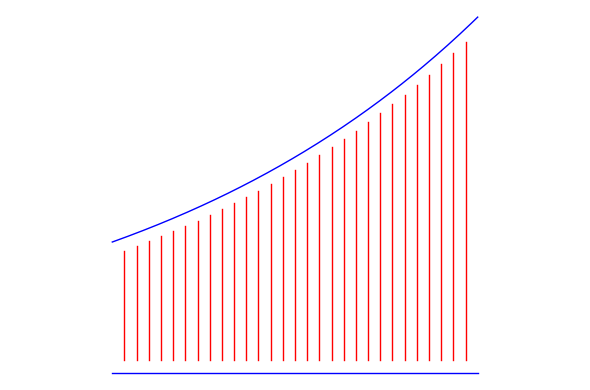
\includegraphics[width=\textwidth]{expcell.png}
      \end{minipage}
      
    \end{enumerate}
  \end{example}
\end{frame}

\begin{frame}{The Pila--Wilkie Theorem}
  \begin{theorem}[Pila--Wilkie]
    Let $\cS$ be an o-minimal structure, let $\epsilon>0$, and let
    $X\subset\IR^m$ be definable in $\cS$. There exists $c(\epsilon,X)>0$
    such that
    \begin{equation*}
      N(X\ssm X^{\mathrm{alg}},T)\le c(\epsilon,X) T^\epsilon \quad\text{for
        all}\quad T\ge 1.
    \end{equation*}
  \end{theorem}

  \begin{itemize}
   \item  $c(\epsilon,X)$ is uniform in families, we
     can replace $X$ by $X_y$ ($y\in\IR^n$)
     when interpeting $X$ as a definable
    family over $\IR^n$.

  \item Pre-o-minimal versions in  dimension $1$ and $2$
    due are to Bombieri--Pila and Pila. The diophantine ``engine'' is
    called \alert{determinant method}.
    
  \item The growth estimate $T^\epsilon$ is best-possible in general.
    Wilkie conjectured a
    poly-logarithmic bound $N(X,T)\le c(X)(\log 3T)^{c'(X)}$ if $\cS=\IRexp$.  
  \end{itemize}
\end{frame}

\begin{frame}{Back to Manin--Mumford}
  Let $A$ be a $g$-dimensional abelian variety defined over $\IC$.
  Recall
  $A(\IC) = \IC^g / \Omega$ with $\Omega$ a rank $2g$ discrete
  subgroup of $\IC^g$. 

  Let $u\colon \IC^g \rightarrow A(\IC)$ be the uniformizaton given by
  theta function and $A\subset\IP^n$. Fix a $\IZ$-basis
  $(\omega_1,\ldots,\omega_{2g})$ of $\Omega$,
  this gives a fundamental domain $\cF\subset\IC^g$ and lets us
  identify $\IC^g$ with $\IR^{2g}$ as $\IR$-vector spaces. 


  \begin{center}
    \begin{minipage}{0.45\linewidth}
      \begin{center}
        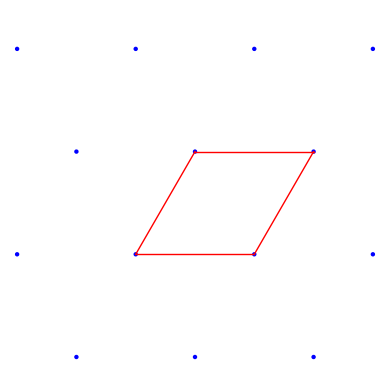
\includegraphics[width=.5\textwidth]{fundamentaldomainav.png}

        Torsion points: $\sum_{i=1}^{2g} \IQ\omega_i$
      \end{center}    
    \end{minipage}$\leadsto$    \begin{minipage}{0.45\linewidth}
      \begin{center}
        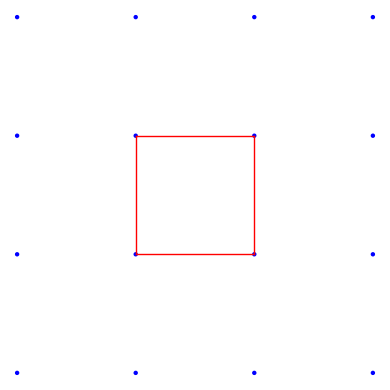
\includegraphics[width=.5\textwidth]{fundamentaldomainav2.png}
        
        Torsion points: $\IQ^{2g}$, Order = height
      \end{center}
    \end{minipage}
  \end{center}

  Let $\tilde u \colon \IR^{2g}\rightarrow A(\IC)$ be the uniformizing map
  in new coordinates. 
\end{frame}

\begin{frame}
  If $V\subset A$ is a subvariety over $\IC$, let $X =
  \tilde u|_{\cF}^{-1}(V(\IC))$.

    \begin{center}
    \begin{minipage}{0.45\linewidth}
      \begin{center}
        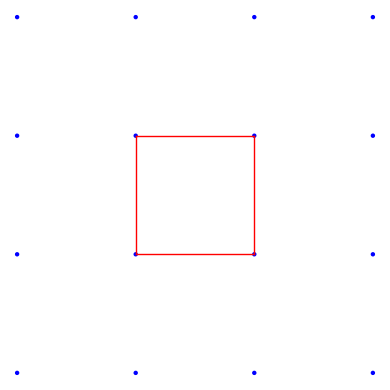
\includegraphics[width=.35\textwidth]{fundamentaldomainav2.png}
        
        Torsion points: $\IQ^{2g}$, Order = height
      \end{center}    
    \end{minipage}$\leadsto$    \begin{minipage}{0.35\linewidth}
      \begin{center}
        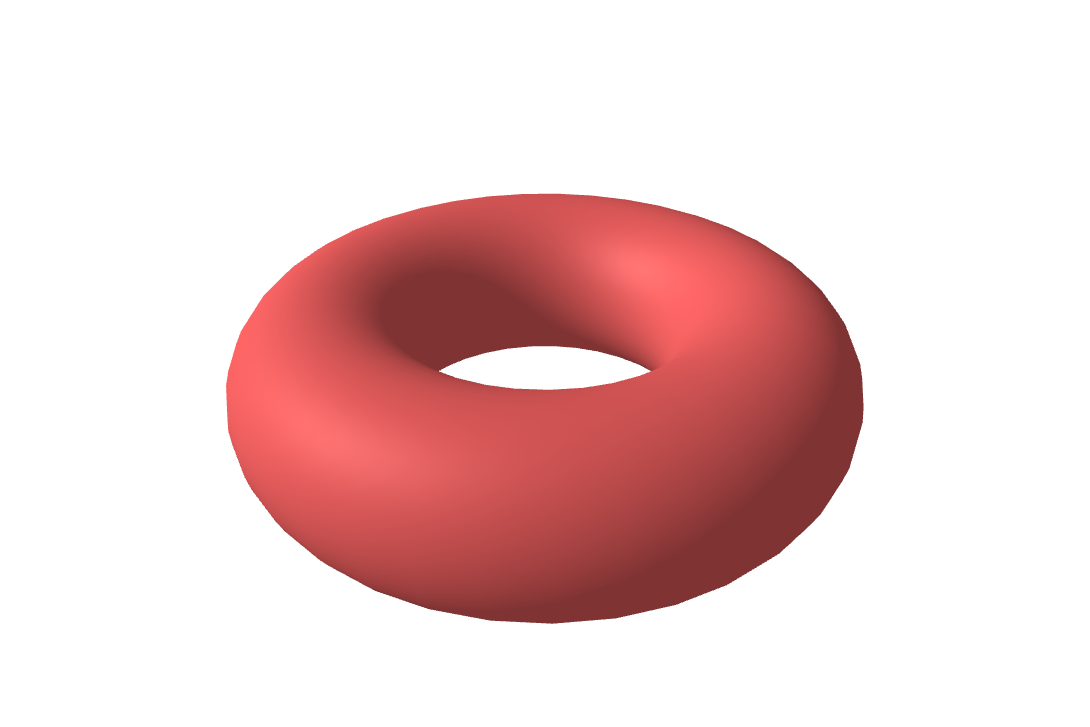
\includegraphics[width=\textwidth]{torus.png}
      \end{center}
    \end{minipage}
  \end{center}

  We will use the Pila--Wilkie Theorem to count rational points on
  $X$.
  To do this we need to understand $X^{\mathrm{alg}}$.
  
  \begin{example}
    Let $B\subset A$ be an abelian subvariety, $\Omega_B = \Omega \cap
    \mathrm{T}_0(B) \subset\IC^g$ has rank $2\dim B$.

    If $B\subset V$ and if $\dim B\ge 1$, then $X$ will contain
    a part of $\mathrm{T}_0(B)$ which is real semi-algebraic. So
    $X^{\mathrm{alg}}\not=\emptyset$.

    We will see that this is essentially the \alert{only} kind of
    contribution to $X^{\mathrm{alg}}$.
  \end{example}
\end{frame}

% \begin{frame}{Back to Monday}
%   Let $C\subset \IG_{\mathrm{m}}^2$ be an algebraic curve and let
%   $$\mathbf{e}(q_1,q_2) = (\exp(2\pi i q_1),\exp(2\pi i q_2)).$$

%   $$\Longrightarrow \quad X=\mathbf{e}^{-1}(C(\IC))\cap [0,1)^2\quad\text{is definable in $\IRan$.}$$

%   \begin{equation*}
%     \text{torsion points on $C(\IC)$} \xleftrightarrow{\text{1-to-1}} \text{rational
%       points on $X$}
%   \end{equation*}

%   Basic idea of Pila--Zannier for the Manin--Mumford Conjecture: apply the counting theorem to $X$.

%   We need to understand the algebraic locus $X^{\mathrm{alg}}$.
% \end{frame}

\section{Functional Transcendence}

\begin{frame}{Classical Transcendence}
  \begin{example}
    \begin{enumerate}
    \item[(i)] Hermite:  $e\not\in\IQbar$, Lindemann: $\pi
      \not\in\IQbar$
    \item[(ii)] Let $z_1,\ldots,z_m\in\IQbar$ be
      $\IQ$-linearly independent. Then
      \begin{equation*}
        \mathrm{trdeg}\,\IQ(\exp(z_1),\ldots,\exp(z_m))/\IQ \ge m,
      \end{equation*}
      follows from the \alert{Lindemann--Weierstrass Theorem}.
      \textit{E.g.} $e$ and $e^{\sqrt{2}} $ are algebraic independent,
      $2\pi i \not\in \IQbar$, $e\not\in\IQbar$.
    \item[(iii)] Gelfond--Schneider: if $a,b\in\IQbar$ with
      $a\not=\{0,1\}$, then $a^b = \exp(b \log a)\not\in \IQbar$.
      \text{E.g.}
      $e^\pi = (-1)^{-i}\not\in\IQbar$.       
    \end{enumerate}
  \end{example}
  
  \begin{conjecture}[Schanuel]
    Let $z_1,\ldots,z_m\in\IC$ be $\IQ$-linearly independent. Then
    \begin{equation*}
      \mathrm{trdeg}\, \IQ(z_1,\ldots,z_m,\exp(z_1),\ldots,\exp(z_m))/\IQ \ge
      m. 
    \end{equation*}
  \end{conjecture}
\end{frame}

\begin{frame}{Ax's Theorem}
  Schanuel's Conjecture is most likely far out of reach.
  It is unknown whether $e+\pi$ is rational or not. 

  But a version for holomorphic maps is known.
  
  \begin{theorem}[Ax]
    Let $\Delta\subset\IC$ be a domain and suppose
    $f_1,\ldots,f_m \colon\Delta \rightarrow\IC$ are holomorphic
    functions that are $\IQ$-linearly independent \alert{modulo
      constants}. Then
    \begin{equation*}
      \mathrm{trdeg}\,\IC(f_1,\ldots,f_m,\exp(f_1),\ldots,\exp(f_m))/\IC \ge
      m+1. 
    \end{equation*}  
  \end{theorem}

  It will help us to better understand $X^{\mathrm{alg}}$. In fact, a
  corollary will be sufficient.
\end{frame}

\begin{frame}
  \begin{corollary}[Ax--Lindemann--Weierstrass]
    Let $C\subset\IC^m$ be a real semi-algebraic curve.
    After replacing $C$ by a non-empty open subset of itself
    $\exp(C)=\{\exp(z) :z\in
    C\}$ is either Zariski dense in
    $(\IC^\times)^m$ or contained in
    the
    translate of a proper algebraic subgroup of $\IG_{\mathrm{m}}^m$.   
  \end{corollary}
  \begin{proof}\renewcommand{\qedsymbol}{}
    \vspace{4cm}
  \end{proof}
\end{frame}

\begin{frame}
  \begin{proof}[Proof continued]
    \vspace{7cm}
  \end{proof}
\end{frame}

\begin{frame}{Conclusion}
  \begin{enumerate}
  \item [(i)]  The height of an element of $\IQ^m$ measures its arithmetic
    complexity.
    There are only finitely many elements in $\IQ^m$ of bounded
    height, this is called the Northcott property.
    
  \item[(ii)] Let $X\subset\IR^m$ be a set definable in some o-minimal
    structure.
    The number of rational points of height $\le T$  outside the
    \alert{algebraic locus} $X^{\mathrm{alg}}$ of $X$ grows at most
    like $O_\epsilon(T^{\epsilon})$ as $T\rightarrow\infty$.
    
    This is the content of the Pila--Wilkie Theorem.
  \end{enumerate}

  
  The Pila--Wilkie tells us something about rational points on the
  \alert{transcendental} part of a definable set.
  It bypasses the difficult questions attached to
  rational points on \alert{algebraic} sets.

  \bigskip
  \begin{displayquote}
    ``Worüber man nicht sprechen kann, darüber muss man schweigen.''
  \end{displayquote}
\end{frame}


\begin{frame}
  \begin{center}
    Thanks for your attention.

    See you tomorrow when we will discuss functional transcendental
    and begin the proof of the Manin--Mumford Conjecture for
    abelian varieties. 
  \end{center}
\end{frame}

\end{document}
